\documentclass[11pt,letterpaper]{article}
\usepackage{fullpage}
\usepackage[top=0.5in, bottom=1.5in, left=1in, right=1in]{geometry}
\usepackage{amsmath,amsthm,amsfonts,amssymb,amscd}
\usepackage{lastpage}
\usepackage{enumerate}
\usepackage{enumitem}
\usepackage{fancyhdr}
\usepackage{graphicx}
\usepackage{listings}
\usepackage{hyperref}
\usepackage{booktabs}
\usepackage{cancel}
\usepackage{physics}
\usepackage{caption,cleveref,colortbl,csquotes,datatool,helvet,mathpazo,multirow,listings,pgfplots,xcolor}

\hypersetup{%
  colorlinks=true,
  linkcolor=blue,
  linkbordercolor={0 0 1}
}

\setlength{\parindent}{0.0in}
\setlength{\parskip}{0.05in}
\setlength{\footnotesep}{1.2\baselineskip}

% edit these
\newcommand\course{AST222H}
\newcommand\Title{Problem Set 3}
\newcommand\Name{Jeff Shen} 
\newcommand\Id{1004911526} 
\newcommand\Date{6 Mar 2020}

\pagestyle{fancyplain}
\headheight 35pt
\lhead{\Name}
\lhead{\Name\\\Id}
\chead{\LARGE \Title}
\rhead{\course \\ \Date}
\lfoot{}
\cfoot{}
\rfoot{\small\thepage}
\pgfplotsset{compat=1.16}
\headsep 1.2em

\begin{document}

% problem 1
\section*{Problem 1}

Given that all stars have the same mass $m$, and $Nm=M$, and all stars have a mean velocity of $V$, the total kinetic energy becomes 
\begin{align*}
    \sum^N_{i=1}\frac{1}{2}m_iv_i^2 &= \frac{1}{2}\sum^N_{i=1}mV^2 \\
    &= \frac{1}{2}mV^2\sum^N_{i=1}1 \\
    &= \frac{1}{2}mV^2N,
\end{align*}

and the potential energy is
\begin{align*}
    -\sum^N_{i=1}\sum^N_{j=1}\frac{Gm_im_j}{|r_i-r_j|} &= -\sum^N_{i=1}\sum^N_{j=1}\frac{Gm^2}{R} \\
    &= -\frac{Gm^2}{R}N^2.
\end{align*}

Using the virial theorem, we find that 
\begin{alignat*}{2}
    &&K &= -\frac{U}{2} \\
    \implies&& \frac{1}{2}NmV^2 &= - \frac{GN^2m^2}{2R} \\
    \implies&& V^2 &= -\frac{GNm}{R} \\ 
    &&&=\frac{GM}{R}
\end{alignat*}

\section*{Problem 2}
\begin{enumerate}[label=(\roman*)]
    \item \hfill

        \begin{parbox}{\linewidth}{
                \centering
                \begin{minipage}[b]{0.45\textwidth}
                    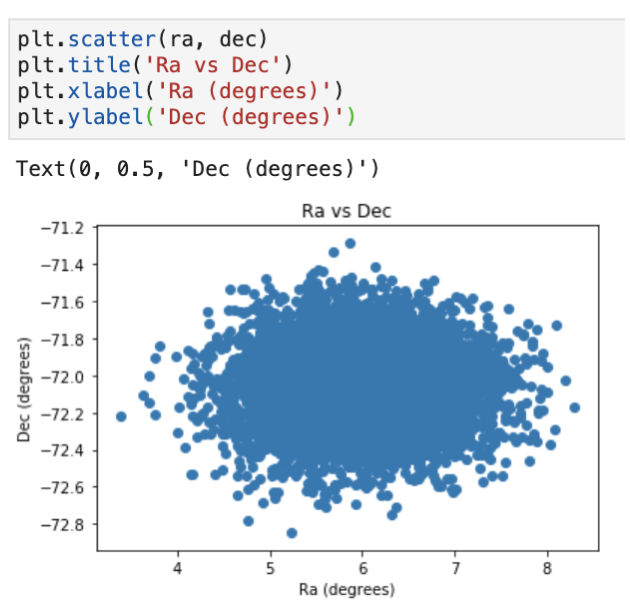
\includegraphics[width=\linewidth]{figures/q21pos.png}
                \end{minipage}
                \hfill
                \begin{minipage}[b]{0.45\textwidth}
                    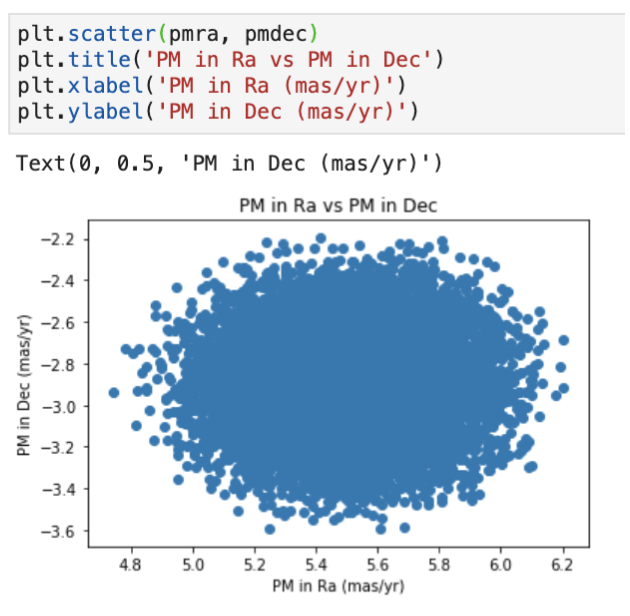
\includegraphics[width=\linewidth]{figures/q21pm.png}
                \end{minipage}
            }
        \end{parbox}

    \item \hfill

        \begin{parbox}{\linewidth}{
                \centering
                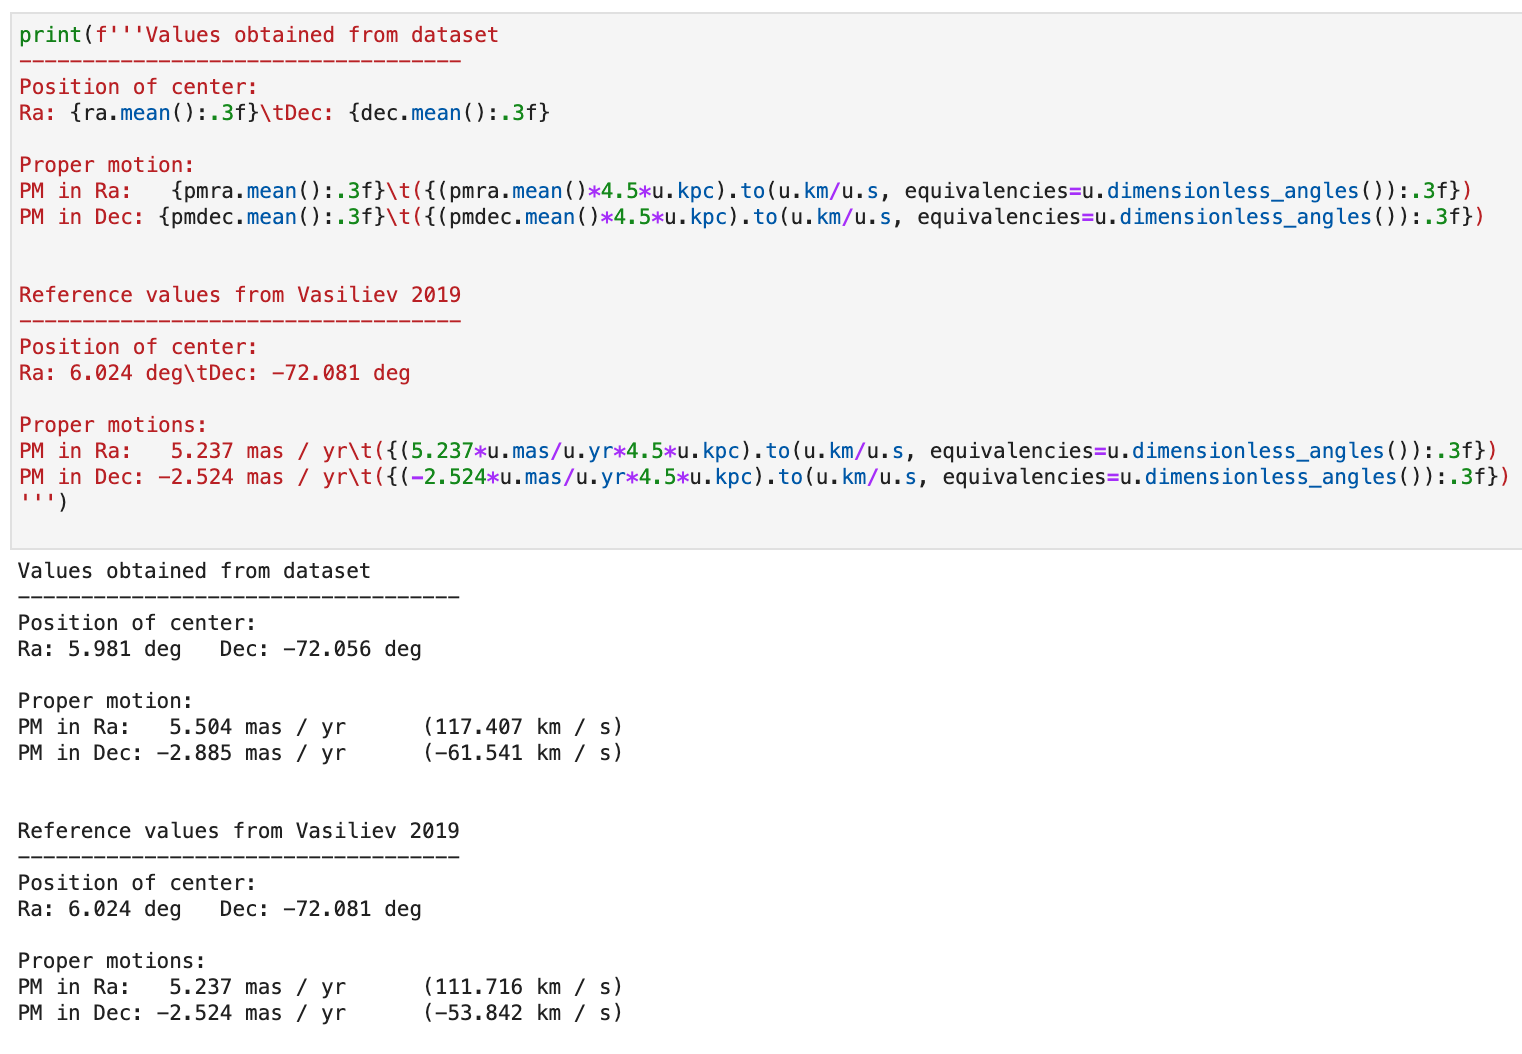
\includegraphics[width=0.9\linewidth]{figures/q22.png}
            }
        \end{parbox}

    \item \hfill

        \begin{parbox}{\linewidth}{
                \centering
                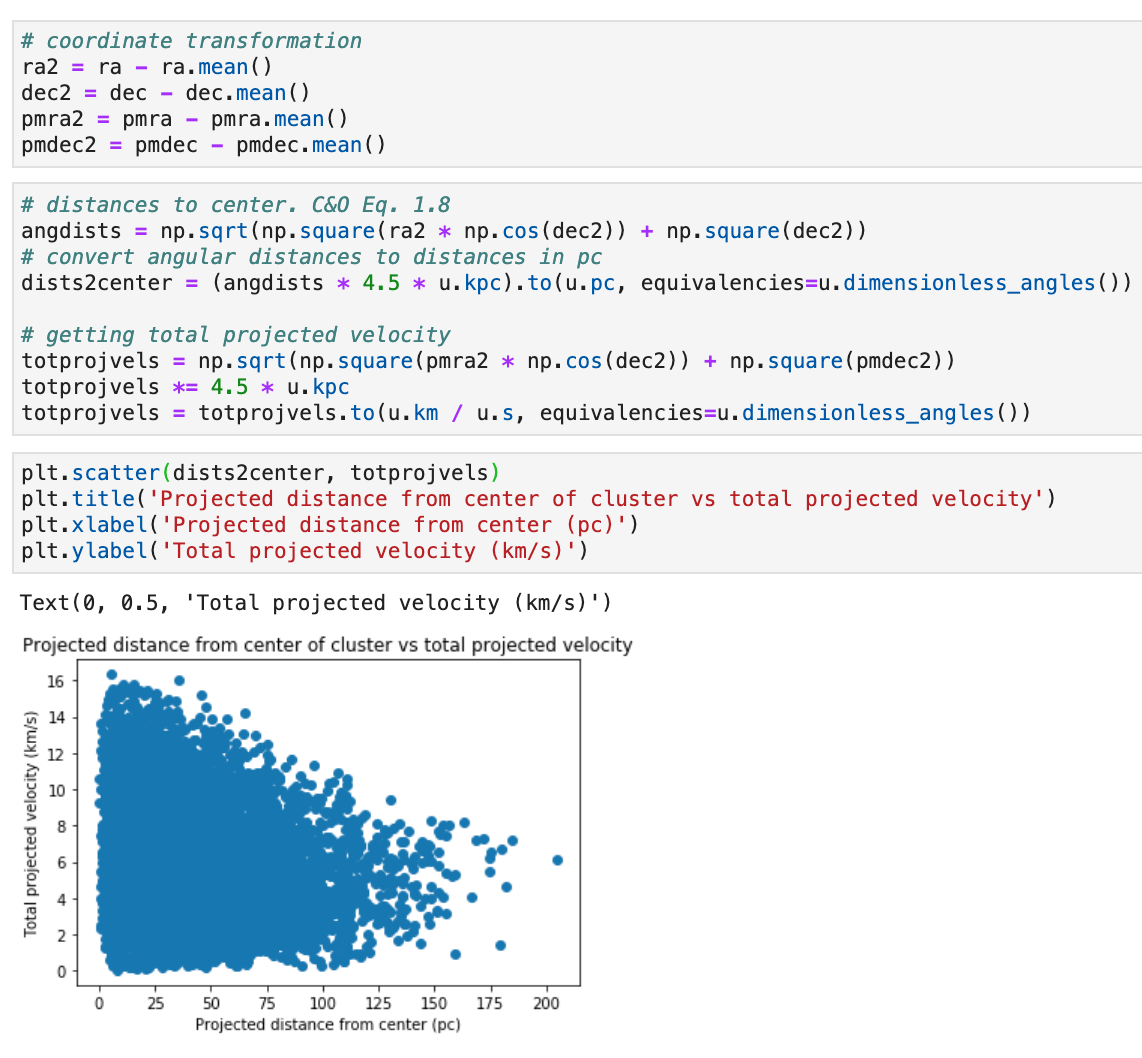
\includegraphics[width=0.8\linewidth]{figures/q23.png}
            }
        \end{parbox}

    \item Velocity is given by Hint 1:
        \begin{align*}
            V = \sqrt{3\sigma_{1D}^2},
        \end{align*}
        where $\sigma_{1D}^2$ is the variance in the projected velocity. The radius is taken to be the maximum of the projected distances from the center of the cluster. 

        \begin{parbox}{\linewidth}{
                \centering
                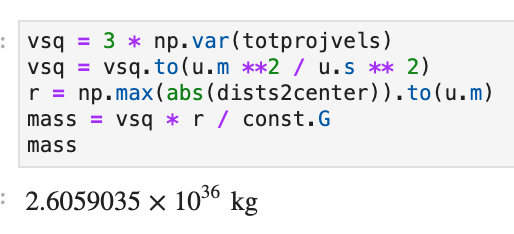
\includegraphics[width=0.5\linewidth]{figures/q24.png}
        }\end{parbox}

    \item \hfill

        \begin{parbox}{\linewidth}{
                \centering
                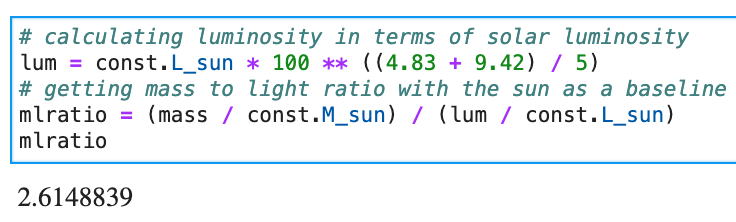
\includegraphics[width=0.75\linewidth]{figures/q25.png}
            }
        \end{parbox}

        The mass-to-light ratio is somewhat low and it seems plausible that 47 Tuc contains very little dark matter. 

    \item The code is the same and won't be shown here. Performing the same analysis, the results for Keanu are as follows:
        \begin{itemize}
            \item mass estimate: $2.23\times 10^{39}~{\rm kg}$
            \item mass-to-light ratio: $99.5~\Upsilon_\odot$
        \end{itemize}
        The high mass-to-light ratio of Keanu indicates that it is dominated by dark matter. 

\end{enumerate}


\newpage
% problem 3
\section*{Problem 3}

\begin{enumerate}[label=(\roman*)]
    \item Solving the lensing equation for $\theta$ gives 
        \begin{align*}
            \beta &= \theta - \frac{\theta_E^2}{\theta^2}\theta \\
            &= \theta - \frac{\theta_E^2}{\theta}.
        \end{align*}
        We multiply both sides of the equation by $\theta$ and solve the quadratic in $\theta$:
        \begin{alignat*}{2}
            &&\theta^2 - \beta\theta - \theta_E^2 &= 0 \\
            \implies&& \theta &= \frac{\beta \pm \sqrt{\beta^2 - 4(-\theta_E^2)}}{2} \\
            &&& = \frac{\beta \pm \sqrt{\beta^2 + 4\theta_E^2}}{2}.
        \end{alignat*}

    \item The Einstein angle for the given parameters is:
        \begin{figure}[!ht]
            \centering
            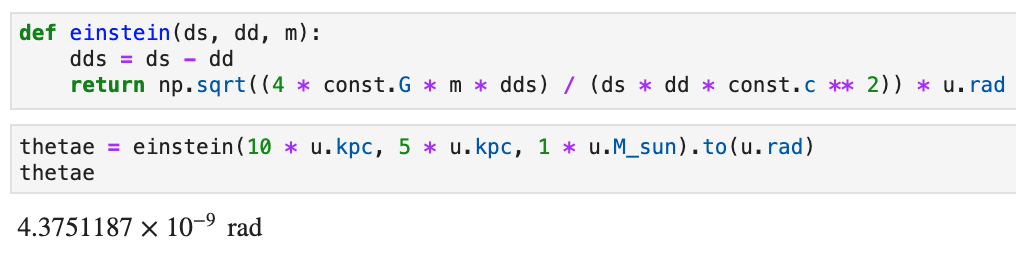
\includegraphics[width=0.7\linewidth]{figures/einstein_angle.png}
        \end{figure}

        For each of the different $\beta$ values (in the order given), using the smallest $|\theta|$, $|\theta|/\theta_E$ is:
        \begin{figure}[!ht]
            \centering
            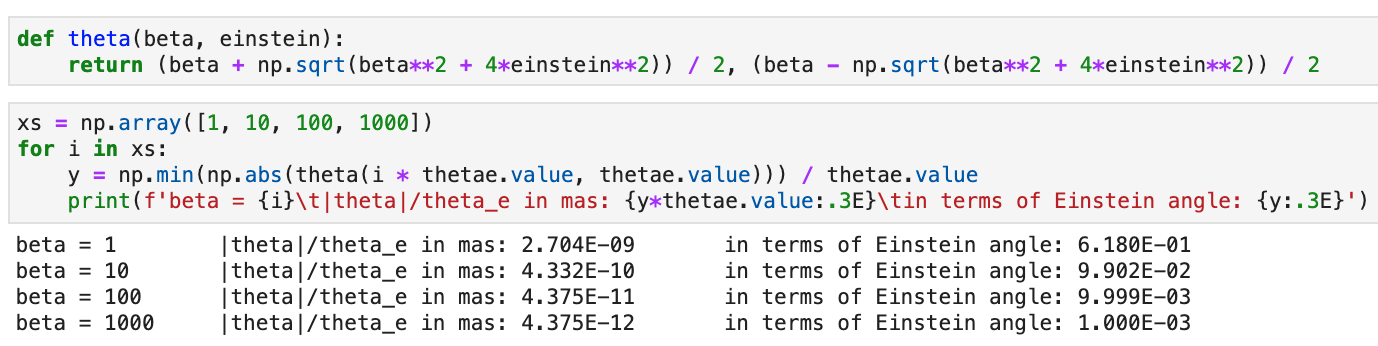
\includegraphics[width=0.9\linewidth]{figures/theta_thetae.png}
        \end{figure}

        As $\beta \rightarrow \infty$, $\theta$ becomes 
        \begin{align*}
            \lim_{\beta\to\infty}\theta &= \lim_{\beta\to\infty}\frac{\beta\pm\sqrt{\beta^2+4\theta_E^2}}{2} \\
            &= \lim_{\beta\to\infty}\frac{\beta\pm\sqrt{\beta^2}}{2} \\
            &= \lim_{\beta\to\infty}\frac{\beta \pm \beta}{2} \\
            \implies \theta &\rightarrow \beta, 0
        \end{align*}

        The smaller solution approaches 0. 

    \item Assuming that the radius of such a star is the same as that of the Sun, and using the small angle approximation, $\beta$, in terms of the previously computed Einstein angle, is\footnote{Physically it doesn't really make sense for $\beta$ to be negative, but this doesn't really matter in terms of calculating distances—if you try to plug the negative result into the formula to calculate $\theta$ (the one from part a) and take the solution with the smaller absolute value, you get the same result as plugging in +970.26.}
        \begin{figure}[!ht]
            \centering
            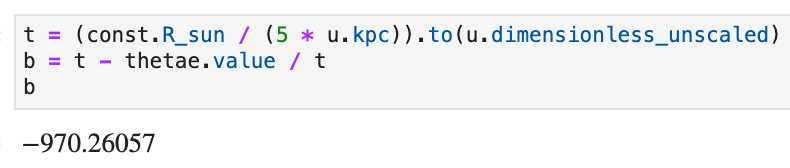
\includegraphics[width=0.8\linewidth]{figures/beta1.png}.
        \end{figure}

        Converting this into mas:
        \begin{figure}[!ht]
            \centering
            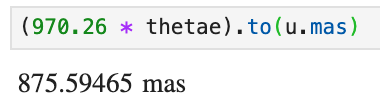
\includegraphics[width=0.4\linewidth]{figures/beta2.png}.
        \end{figure}

    \item Assume that there are roughly $10^{11}$ stars in the sky (the number of stars in the galaxy), and that they are uniformly distributed. Also assume that you can only see half of the sky (the ground is blocking the other half). The area of the sky is $4\pi$ steradians (sr), so the area of the visible portion is $2\pi$ sr. Then the "density" of stars in the sky is 
        \begin{align*}
            \frac{5\times 10^{10}~{\rm stars}}{2\pi~{\rm sr}} = 7.958\times 10^{9}~{\rm stars/sr}.
        \end{align*}
        The reciprocal of this gives the area of the sky taken up by each star:
        \begin{align*}
            \frac{1}{7.96\times 10^{9}~{\rm stars/sr}} = 1.257\times 10^{-10}~{\rm sr/star}.
        \end{align*}
        Ignoring that circles have a maximum packing density of 0.9069 (or ignoring overlaps if the circles are forced closer together), assume that the area taken up by each star is in the shape of a circle. Using this assumption, we can calculate the diameter of each star from the area:
        \begin{align*}
            r = \sqrt{\frac{A}{\pi}} = \sqrt{\frac{1.257\times 10^{-10}~{\rm sr}}{\pi}} = 1.121\times 10^{-5}~{\rm rad} \\
            \implies d = 2r = 2.242\times 10^{-5}~{\rm rad} \simeq 4.624~{\rm mas}.
        \end{align*}
        This is smaller than the result we found in the previous part, and this suggests that, for a typical lens-source system in the sky, there is no second image. 

    \item We take the limit of the magnification as $\beta\to\infty$:
        \begin{align*}
            \lim_{\beta\to\infty}\mu &= \lim_{\beta\to\infty}\frac{1}{4}\left(\frac{\beta}{\sqrt{\beta^2 + 4\theta_E^2}} + \frac{\sqrt{\beta^2 + \4\theta_E^2}}{\beta} \pm 2\right) \\
            &= \lim_{\beta\to\infty}\frac{1}{4}\left(\frac{\beta}{\sqrt{\beta^2}} + \frac{\sqrt{\beta^2}}{\beta} \pm 2\right) \\
            &= \lim_{\beta\to\infty}\frac{1}{4}\left(1 + 1 \pm 2\right) \\
            \implies \mu &\rightarrow 1, 0
        \end{alignat*}

        The magnification of the second image approaches 0 (i.e. the image disappears). 

\end{enumerate}


\end{document}
